We evaluate the performance of \appName{} by running it on the Amazon EC2 cloud, which provides a web interface through which images for virtual machines can be created, managed, and launched.
We create one image containing our load balancer and one image containing code for the solver machine.
We need to launch only the load balancer image, which will launch solver instances on its own depending on workload.
Since the solver machines need to accept requests from the load balancer, we rented an \textit{Elastic IP} for the load balancer, which means that its IP does not change between launches.
We use this IP address to make Sudoku requests to the load balancer
In the instance overview of the EC2 web interface we can see the state (starting, running, stopping, stopped, terminated) of all instances.

The workload is generated by a Java program running locally on our own machines.
It contains a large list of partially completed puzzles.
Within random intervals the program selects a random puzzle from the list a makes a GET request to the load balancer.   
The workload program is multithreaded to allow new requests to be made while others are still active.
Alongside the workload generation there is a monitoring thread which inspects and logs data from the load balancer such as the number of active machines and resource usage.

Figure~\ref{fig:exp:load} shows the workload and the number of solver machines over a period of time.
Machines allocated when the workload is high, and they are terminated when it drops. 

\begin{figure}[H]
	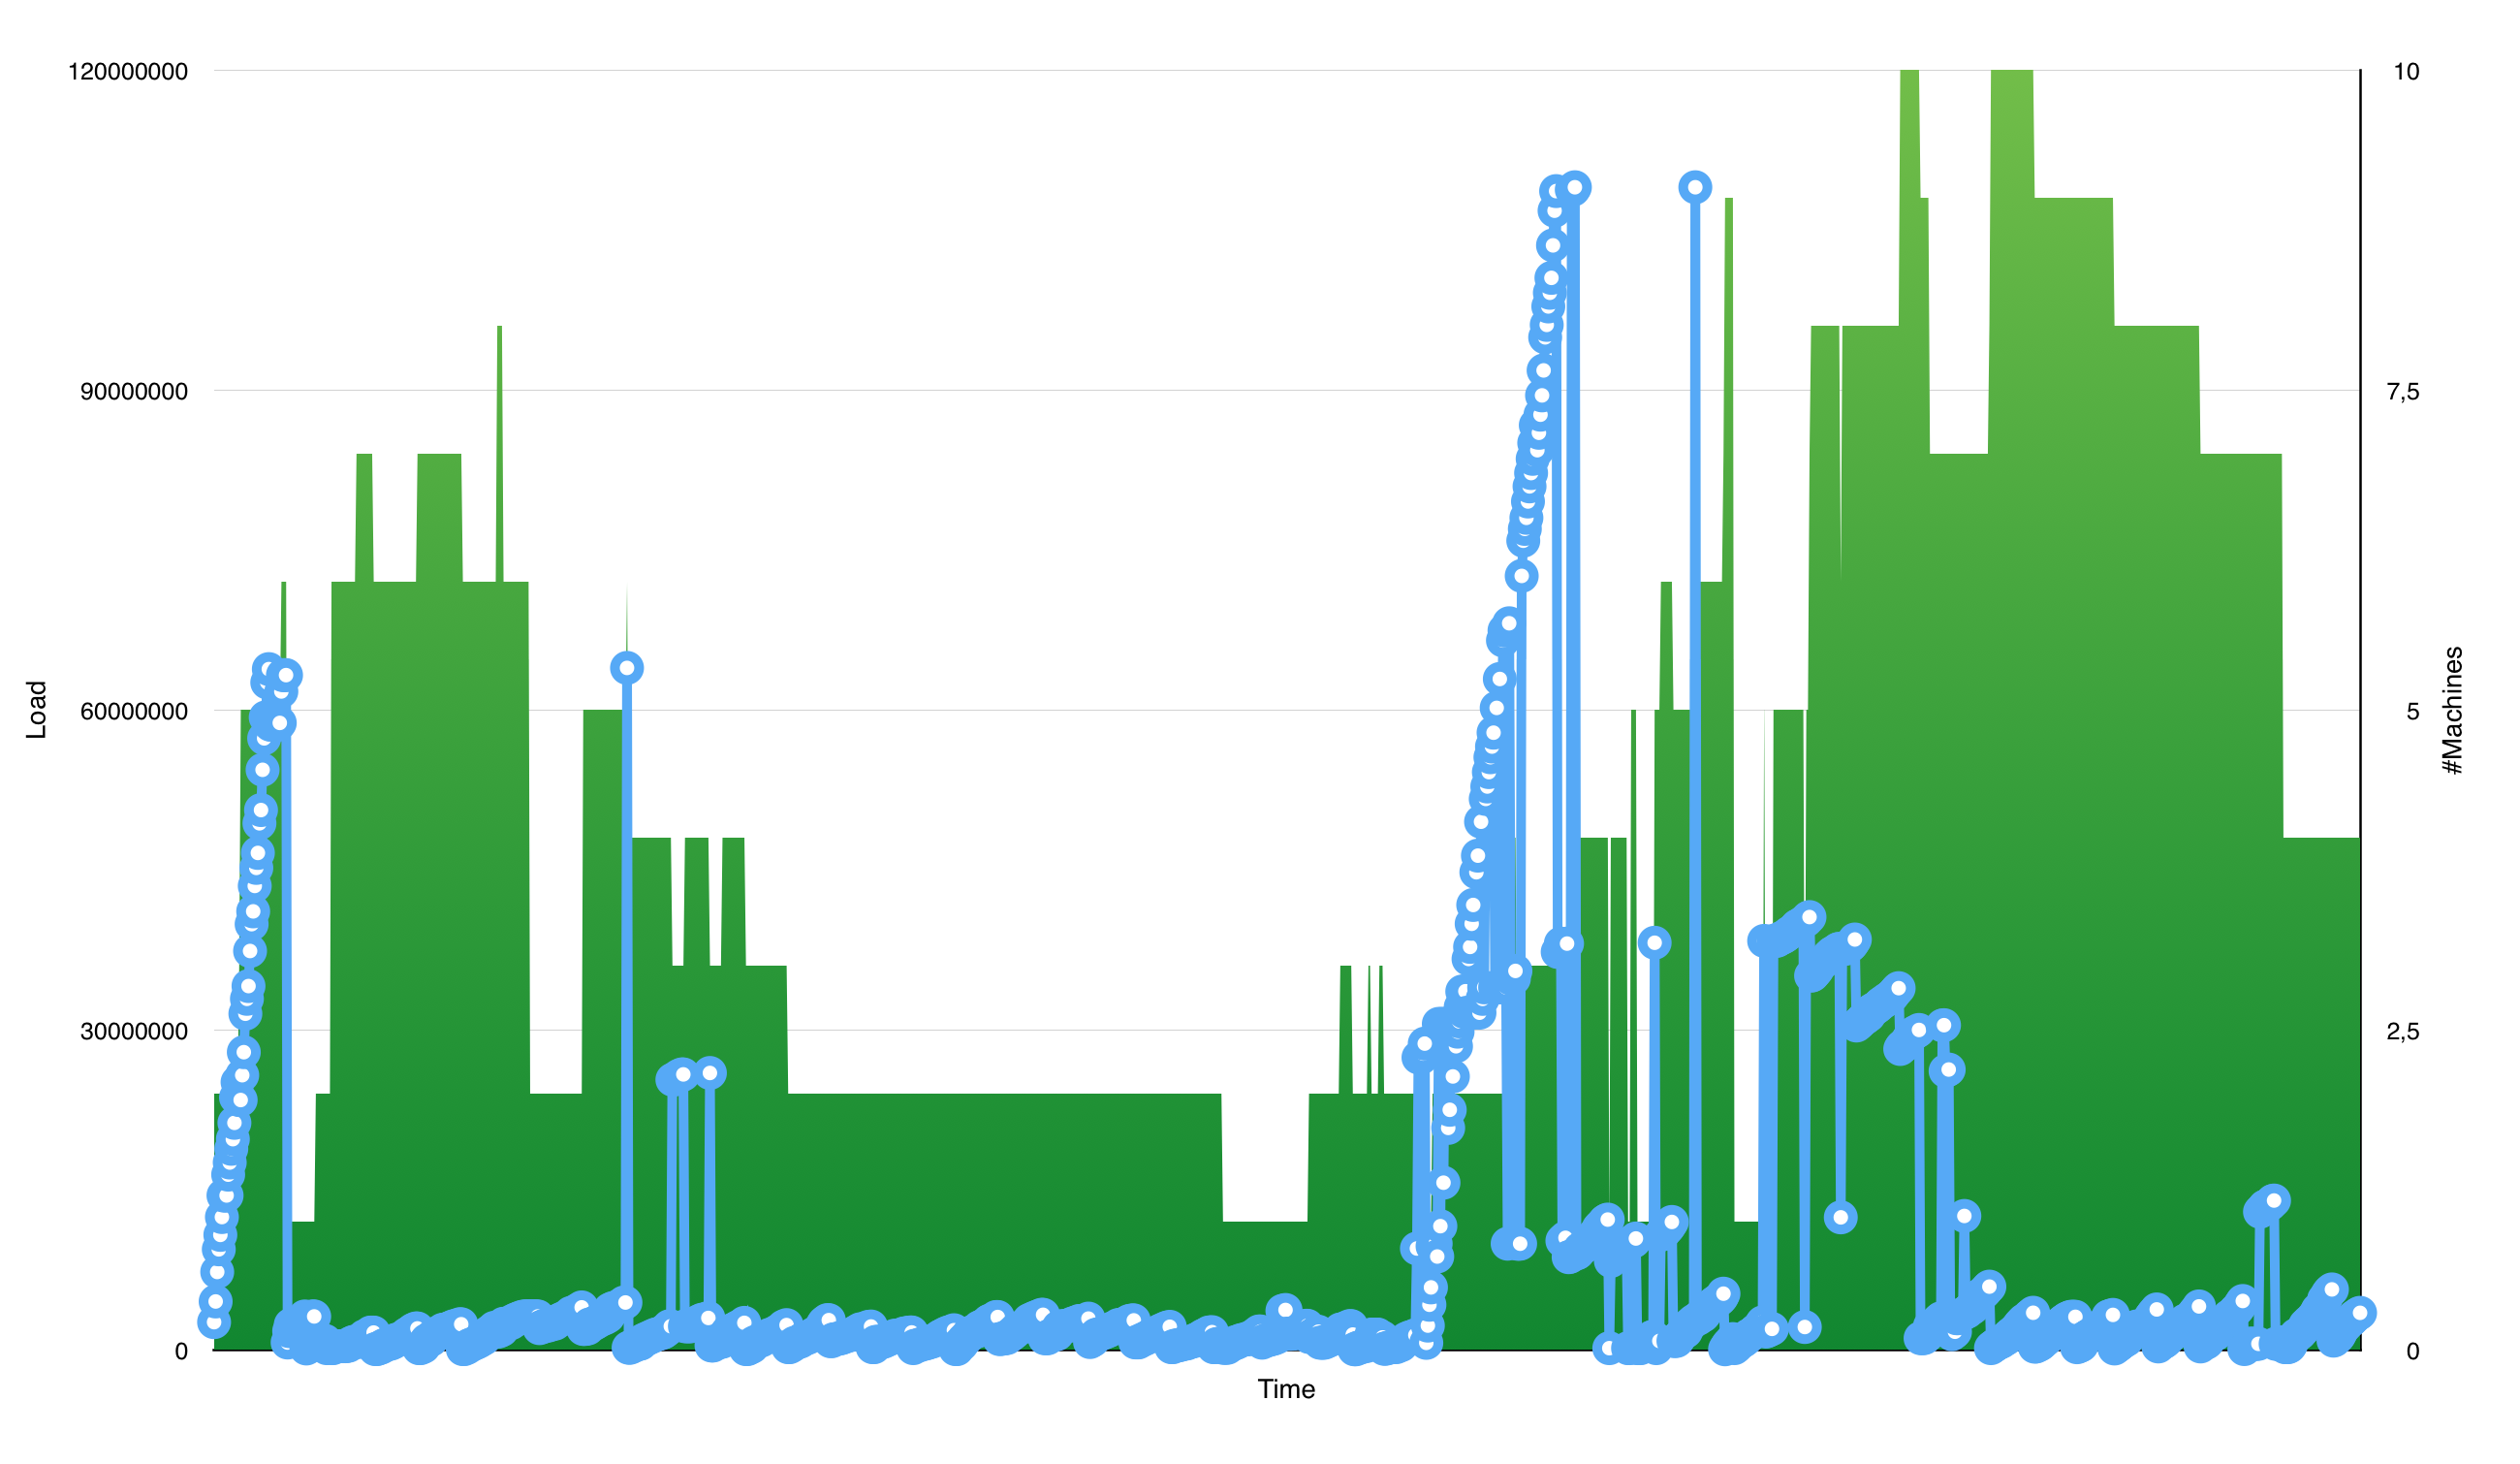
\includegraphics[width=\linewidth]{load_and_machines}
	\caption{The workload(blue) and the number of machines(green) plotted over time}
	\label{fig:exp:load}
\end{figure}

The workload is the sum of the workloads for all application servers.
Each 30 seconds, when the clean up task is run, the load of each server will decrease by its typical max load.
In the plot, if the total workload drops, but not all the way to zero, this means that the total workload was too high to handle and a new instance will be started.

Figure~\ref{fig:exp:response} shows the distribution of the response time the end user experiences when making a request. Data for this experiment was gathered during varying workload. It shows that although there is some variation, the delay is always less than 60 milliseconds.

\begin{figure}[H]
	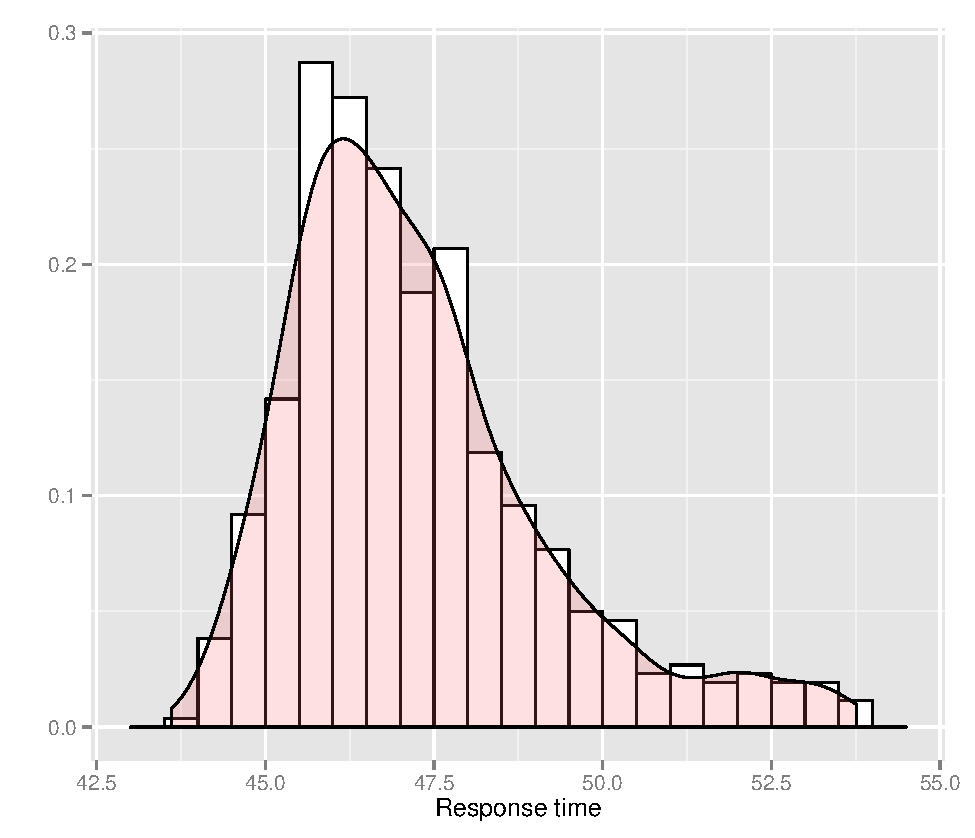
\includegraphics[width=\linewidth]{hist_response_time}
	\caption{Distribution of the response time in milliseconds of the server, with outliers removed}
	\label{fig:exp:response}
\end{figure}
